\documentclass[conference]{IEEEtran}
\IEEEoverridecommandlockouts
% The preceding line is only needed to identify funding in the first footnote. If that is unneeded, please comment it out.
%Template version as of 6/27/2024

\usepackage{cite}
\usepackage{amsmath,amssymb,amsfonts}
\usepackage{graphicx}
\usepackage{textcomp}
\usepackage{xcolor}
\usepackage{url} 
\def\BibTeX{{\rm B\kern-.05em{\sc i\kern-.025em b}\kern-.08em
    T\kern-.1667em\lower.7ex\hbox{E}\kern-.125emX}}
\usepackage[brazil]{babel}
\usepackage{algorithm}
\usepackage{algorithmicx}
\usepackage{algpseudocode}
\usepackage{subcaption}
\usepackage{multirow}
\usepackage{booktabs}
\usepackage{amsmath}  % já está incluído no seu caso
\allowdisplaybreaks   % permite quebra de página em ambientes align, gather, etc.

\begin{document}

\def\portugues{1}
\selectlanguage{brazil}

\title{Aprimoramento de Metaheurísticas para Otimização da Cadeia de Suprimentos de Pistache}

\author{\IEEEauthorblockN{1\textsuperscript{st} Raissa Gon\c{c}alves Diniz}
\IEEEauthorblockA{\textit{Operations Research and Complex Systems Laboratory} \\
\textit{Universidade Federal de Minas Gerais}\\
Belo Horizonte, Brasil \\
raissagd@ufmg.br}
\and
\IEEEauthorblockN{2\textsuperscript{nd} Andr\'e Costa Batista}
\IEEEauthorblockA{\textit{Departamento de Engenharia Elétrica} \\
\textit{Universidade Federal de Minas Gerais}\\
Belo Horizonte, Brasil \\
andre-costa@ufmg.br}
}

\maketitle

\begin{abstract}
    As cadeias de suprimentos desempenham um papel fundamental na indústria agrícola, especialmente no caso de culturas de alto valor, como o pistache, onde uma gestão 
    eficiente pode impulsionar o crescimento econômico e promover a sustentabilidade. Embora pesquisas anteriores tenham explorado estratégias de otimização para essas 
    cadeias, a maioria dos estudos concentra-se no uso de algoritmos populacionais para enfrentar esses desafios. Neste trabalho, propomos a aplicação do algoritmo de 
    Busca em Vizinhança Variável (Variable Neighborhood Search - VNS) e avaliamos seu desempenho em comparação com uma metaheurística populacional, especificamente o Algoritmo Genético (Genetic Algorithm - GA). 
    Os resultados mostram que o VNS apresenta consistentemente um desempenho superior ao GA, tanto em termos de eficiência computacional quanto de qualidade das soluções, especialmente 
    em instâncias de maior porte. Esses achados destacam o potencial do método proposto como uma abordagem eficaz para a otimização de cadeias de suprimentos.
\end{abstract}


\begin{IEEEkeywords}
    Otimização de Cadeias de Suprimentos, Metaheurísticas, Busca em Vizinhança Variável, Sustentabilidade.
\end{IEEEkeywords}

% %===============================================================================
\section{Introdução}
\label{sec:intro1}
A agricultura desempenha um papel fundamental no desenvolvimento econômico, contribuindo não apenas para a segurança alimentar, mas também para as exportações e o crescimento industrial. 
Entre as culturas de alto valor, os pistaches se destacam no comércio internacional, com os Estados Unidos, a Turquia e o Irã liderando a produção global \cite{b22}. 
A gestão eficiente de cadeias de suprimentos é essencial para manter a qualidade dos produtos, reduzir impactos ambientais e garantir uma distribuição eficaz. Um dos principais desafios na 
produção de pistache é o manejo dos subprodutos, como cascas e resíduos da polpa, que, se descartados de forma inadequada, podem comprometer a qualidade do solo e gerar riscos à saúde 
devido à contaminação por aflatoxinas produzidas por fungos \cite{b26}. Estratégias sustentáveis de gestão de resíduos, como compostagem e produção de biogás, têm sido 
exploradas para mitigar esses problemas, conforme discutido por \cite{b6}.

Falhas na cadeia de suprimentos exercem impacto significativo tanto na qualidade dos produtos quanto nas operações comerciais. Estudos anteriores, como o de \cite{b2}, investigaram técnicas 
de otimização baseadas em Algoritmos Genéticos (Genetic Algorithm - GA) e outras meta-heurísticas evolucionárias para a logística do pistache. No entanto, muitas dessas comparações se baseiam apenas 
nas melhores soluções encontradas, sem uma validação estatística robusta que comprove a superioridade dos resultados. Além disso, ainda há debate sobre a influência real das 
diferenças entre meta-heurísticas bioinspiradas na qualidade das soluções obtidas.

Neste estudo, propõe-se a otimização da cadeia de suprimentos do pistache utilizando a metaheurística Busca em Vizinhança Variável (Variable Neighborhood Search - VNS), que é amplamente reconhecida 
por sua eficácia na resolução de problemas combinatórios complexos com baixa necessidade de parametrização. O modelo matemático utilizado é baseado na formulação mista linear proposta por \cite{b2} 
para a logística direta e reversa, que foca na minimização de custos e na redução de impactos ambientais por meio do reaproveitamento de subprodutos. A principal contribuição deste trabalho está na 
aplicação do VNS a esse modelo, avaliando seu desempenho em comparação com o Algoritmo Genético (GA). Os resultados demonstram que o VNS apresenta vantagens em termos de qualidade 
das soluções e tempo computacional. Embora o uso de metaheurísticas para otimização de cadeias de suprimentos não seja novo, a aplicação específica do VNS neste contexto oferece uma alternativa 
interessante e promissora, especialmente em problemas de maior escala e complexidade. Essa abordagem pode contribuir para o aprimoramento da eficiência na gestão de cadeias de suprimentos agrícolas, 
mantendo a sustentabilidade e otimizando os custos operacionais.

A estrutura deste artigo organiza-se da seguinte forma: a Seção~\ref{sec:problem-def1} apresenta a definição do problema, descrevendo a estrutura da cadeia de suprimentos e os 
objetivos de otimização. A Seção~\ref{sec:heuristic1} detalha a abordagem heurística, explicando a metodologia VNS e sua implementação. A Seção~\ref{sec:experiments1} compara os 
resultados experimentais entre VNS e GA. Por fim, a Seção~\ref{sec:conclusion1} apresenta as principais conclusões e direções para pesquisas futuras.

%===============================================================================
\section{Definição do Problema}
\label{sec:problem-def1}

A rede logística proposta por \cite{b2}, ilustrada na Figura~\ref{fig:supplychain}, descreve o fluxo de produtos e subprodutos ao longo da cadeia de suprimentos do pistache. O processo tem 
início com os produtores (\(i\)), que enviam os pistaches colhidos aos centros de processamento (\(j\)). Nesses centros, os pistaches são transformados em três componentes principais: 
pistaches de casca aberta, sementes cruas e resíduos orgânicos.

Cada um desses componentes segue fluxos específicos. Os pistaches de casca aberta são encaminhados às fábricas de pistache (\(k\)), que os processam e os distribuem aos clientes finais (\(n1\)). 
As sementes cruas são enviadas aos centros de extração de óleo (\(e\)), responsáveis pela produção de óleo de pistache, o qual é direcionado tanto a clientes finais (\(n2\)) quanto às fábricas de cosméticos
(\(s\)). Estas, por sua vez, processam o óleo em produtos cosméticos que são fornecidos aos respectivos consumidores (\(n3\)). Os resíduos orgânicos gerados no processamento inicial são destinados aos centros 
de compostagem (\(q\)), onde são transformados em composto, posteriormente distribuído aos clientes de compostagem (\(m\)).

Embora, em termos práticos, o composto produzido possa ser reutilizado pelos próprios produtores agrícolas, estabelecendo um sistema de circuito fechado, o modelo matemático adotado não representa 
explicitamente essa retroalimentação. Em vez disso, os clientes de composto não estão diretamente associados aos produtores originais, caracterizando um ciclo de feedback implícito. Essa abordagem, 
já adotada em trabalhos anteriores (\hspace{-0.03em}\cite{b11,b19,b20}), preserva a simplicidade estrutural do modelo. No entanto, a inclusão de uma modelagem rigorosa desse circuito de retorno 
representa uma direção promissora para investigações futuras, especialmente no contexto de cadeias de suprimentos sustentáveis.

\begin{figure}
  \begin{center}
      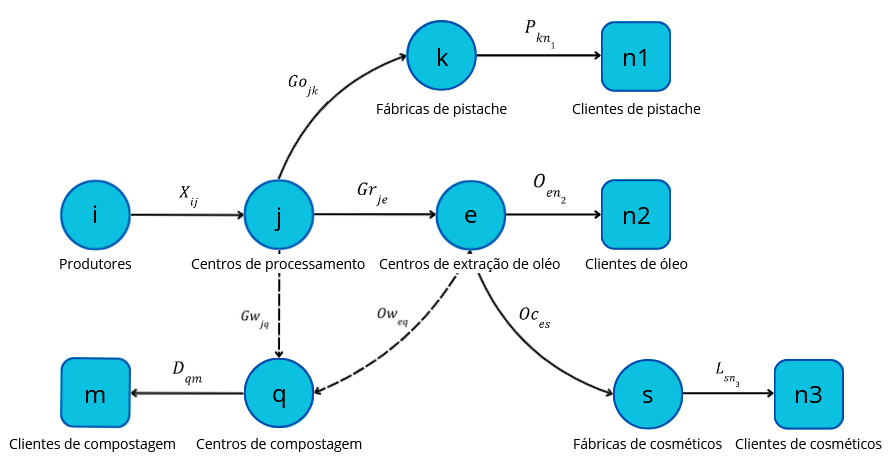
\includegraphics[width=8.4cm]{./imgs/fluxo_pt.PNG}
      \caption{Estrutura da cadeia de suprimentos do pistache proposta.}
      \label{fig:supplychain}
  \end{center}
\end{figure}

O problema linear misto visa minimizar os custos totais \eqref{eq:custo}, incluindo custos de abertura, produção e transporte, sob as seguintes restrições de capacidade e demanda, não tolerando escassez (ver
mais detalhes sobre as variáveis na Tabela 5 de \cite{b2}):

\begin{align}
    \min &\ z_1 + z_2 + z_3 \label{eq:custo}\\
    \text{s.t.:} \quad & \sum\limits_{j=1}^J X_{ij} \le Cpa_i, \quad \forall i \in I \label{eq:restricao1}\\
    & \sum\limits_{i=1}^I X_{ij} \le Cpu_j\times U_j, \quad \forall j \in J \label{eq:restricao2}\\
    & \sum\limits_{e=1}^E Ow_{eq} + \sum\limits_{j=1}^J Gw_{jq} \le Cpy_q \times Y_q, \quad \forall q \in Q \label{eq:restricao3}\\
    & \sum\limits_{j=1}^J Go_{jk} \le Cpw_k\times W_k, \quad \forall k \in K \label{eq:restricao4}\\
    & \sum\limits_{j=1}^J Gr_{je} \le Cpr_e\times R_e, \quad \forall e \in E \label{eq:restricao5}\\
    & \sum\limits_{e=1}^E O_{en_2} \le Cpv_s\times V_s, \quad \forall s \in S \label{eq:restricao6}\\
    & \sum\limits_{k=1}^K Go_{jk} + \sum\limits_{e=1} Gr_{je} + \sum\limits_{q=1}^Q Gw_{jq} \le \sum\limits_{i=1} X_{ij}, \quad \forall j \in J \label{eq:restricao7} \\
    & \sum\limits_{k=1}^K Go_{jk} = (1-\beta) \sum\limits_{i=1}^I X_{ij}\theta_1, \quad \forall j\in J \label{eq:restricao8} \\
    & \sum\limits_{e=1}^K Gr_{je} = (1-\beta) \sum\limits_{i=1}^I X_{ij}\theta_2, \quad \forall j\in J \label{eq:restricao9} \\
    & \sum\limits_{q=1}^Q Gw_{jq} = \sum\limits_{i=1}^I X_{ij}\theta_3, \quad \forall j\in J \label{eq:restricao10} \\
    & \theta_1 + \theta_2 + \theta_3 = 1 \label{eq:restricao11} \\
    & \sum\limits_{n_1=1}^{N_1} P_{kn_1} \le \sum\limits_{j=1}^J Go_{jk} \times \gamma k, \quad \forall k \in K \label{eq:restricao12} \\
    & \sum\limits_{n_2=1}^{N_2} O_{en_2} + \sum\limits_{s=1}^S Oc_{es} \le \sum\limits_{j=1} Gr_{je}\times(1-\lambda), \quad \forall e\in E \label{eq:restricao13} \\
    & \sum\limits_{q=1}^{Q} Ow_{eq} \le \sum\limits_{j=1}^J Gr_{je} \times \lambda, \quad \forall e \in E \label{eq:restricao14} \\
    & \sum\limits_{n_3=1}^{N_3} L_{sn_1} \le \sum\limits_{e=1}^E Oc_{es} \times \gamma s, \quad \forall s \in S \label{eq:restricao15} \\
    & \sum\limits_{m=1}^M D_{qm} \le \left(\sum\limits_{j=1}^J Gw_{jq} + \sum\limits_{e=1}^E Ow_{eq} \right) \times \gamma q, \quad \forall q \in Q \label{eq:restricao16} \\
    & \sum\limits_{k=1}^K P_{kn_1} \ge Dp_{n_1}, \quad \forall n_1 \in N_1 \label{eq:restricao17}\\
    & \sum\limits_{e=1}^E O_{en_2} \ge Du_{n_2}, \quad \forall n_2 \in N_2 \label{eq:restricao18}\\
    & \sum\limits_{s=1}^S L_{sn_3} \ge Ds_{n_3}, \quad \forall n_3 \in N_3 \label{eq:restricao19}\\
    & \sum\limits_{q=1}^Q D_{qm} \le Dc_{m}, \quad \forall m \in M \label{eq:restricao20}
\end{align}

    
\begin{itemize}
\item A função objetivo \eqref{eq:custo} minimiza os custos totais da cadeia de suprimentos, incluindo custos de abertura, transporte e produção. Os custos são divididos em três componentes: 
$z_1$ \eqref{eq:custo1}, $z_2$ \eqref{eq:custo2}, e $z_3$ \eqref{eq:custo3}, que representam os custos de abertura de instalações, transporte e produção, respectivamente, conforme mostrado nas seguintes equações:
\end{itemize}

\begin{align}
  z_1 &= \sum_{j=1}^J Fu_j \cdot U_j 
      + \sum_{q=1}^Q Fy_q \cdot Y_q 
      + \sum_{k=1}^{K} Fw_k \cdot W_k \notag \\
      &\quad + \sum_{e=1}^{E} Fr_e \cdot R_e
      + \sum_{s=1}^S Fv_s \cdot V_s
      \label{eq:custo1}
\end{align}

\begin{align}
  z_2 &= \sum_{i=1}^I\sum_{j=1}^J CI_i \cdot X_{ij} 
      + \sum_{j=1}^J\sum_{k=1}^K Cu_{1j} \cdot Go_{jk} \notag \\
      &\quad + \sum_{j=1}^J\sum_{e=1}^E Cu_{2j} \cdot Gr_{je} 
      + \sum_{q=1}^Q\sum_{m=1}^M Cy_q \cdot D_{qm} \notag \\
      &\quad + \sum_{k=1}^K\sum_{n_1=1}^{N_1} Cw_k \cdot P_{kn_1} \notag \\
      &\quad + \sum_{e=1}^E Cr_e \cdot \left( \sum_{n_2=1}^{N_2} O_{en_2} 
      + \sum_{s=1}^S Oc_{es} \right) \notag \\
      &\quad + \sum_{s=1}^S\sum_{n_3=1}^{N_3} Cv_s \cdot L_{sn_3}
      \label{eq:custo2}
\end{align}

\begin{align}
  z_3 &= \sum_{i=1}^I\sum_{j=1}^J CX_{ij} \cdot X_{ij} 
      + \sum_{j=1}^J\sum_{k=1}^K CK_{jk} \cdot Go_{jk} \notag \\
      &\quad + \sum_{j=1}^J\sum_{q=1}^Q CJ_{jq} \cdot Gw_{jq}
      + \sum_{e=1}^E\sum_{s=1}^S CS_{es} \cdot Oc_{es} \notag \\
      &\quad + \sum_{e=1}^E\sum_{n_2=1}^{N_2} CN_{en_2} \cdot Oc_{en_2}
      + \sum_{e=1}^E\sum_{q=1}^Q CQ_{eq} \cdot Ow_{eq} \notag \\
      &\quad + \sum_{s=1}^S\sum_{n_3=1}^{N_3} Cl_{sn_3} \cdot L_{sn_3}
      + \sum_{k=1}^K\sum_{n_1=1}^{N_1} Cp_{kn_1} \cdot P_{kn_1} \notag \\
      &\quad + \sum_{q=1}^Q\sum_{m=1}^M Cd_{qm} \cdot D_{qm}
      \label{eq:custo3}
\end{align}

\begin{itemize}
  \item As variáveis $R_j$, $Y_q$, $W_k$, $Z_e$ e $V_s$ são binárias e determinam se certos elementos do modelo estão ativos. Por exemplo, $R_j = 1$ indica que a instalação $j$ está operacional, e $R_j = 0$ caso contrário. As demais variáveis do modelo são contínuas e não negativas, representando valores reais maiores ou iguais a zero. Essas variáveis modelam fluxos, quantidades e outros fatores mensuráveis dentro do sistema.
  
  \item As restrições \eqref{eq:restricao1}-\eqref{eq:restricao6} tratam das limitações de capacidade e demanda de cada instalação na cadeia de suprimentos. Em particular, a restrição \eqref{eq:restricao1} limita a quantidade de produtos transportados dos produtores para os centros de distribuição. Já as restrições \eqref{eq:restricao2}-\eqref{eq:restricao6} garantem que as quantidades enviadas para os centros de processamento, compostagem, fábricas de pistache, centros de extração de óleo e fábricas de cosméticos não ultrapassem as capacidades dessas instalações.
  
  \item A quantidade de produtos enviados de qualquer instalação não deve ultrapassar os pedidos recebidos por essa instalação. Consequentemente, a restrição \eqref{eq:restricao7} estabelece que a quantidade de produtos expedidos de um centro de processamento deve ser menor ou igual à quantidade recebida por outras instalações. As restrições \eqref{eq:restricao8}-\eqref{eq:restricao11} definem as quantidades de pistaches de casca aberta, sementes cruas e resíduos gerados durante o processo de descascamento em cada centro de processamento. De forma similar, as restrições \eqref{eq:restricao12}-\eqref{eq:restricao16} regem os fluxos dentro das fábricas de pistache, centros de extração de óleo, fábricas de cosméticos e centros de compostagem.  
  
  \item Por fim, para garantir que a demanda dos clientes seja atendida, as restrições \eqref{eq:restricao17}-\eqref{eq:restricao20} asseguram que as quantidades de produtos entregues aos clientes de pistache, óleo de pistache, cosméticos e composto satisfaçam ou superem suas respectivas demandas.
\end{itemize}

%===============================================================================
\section{Metodologia}
\label{sec:heuristic1}

Esta seção apresenta a metodologia utilizada para resolver o problema de otimização, empregando codificação baseada em prioridade \cite{b12} e o algoritmo VNS. A codificação 
baseada em prioridade ordena as variáveis de decisão para explorar o espaço de soluções mantendo a viabilidade, enquanto o VNS alterna entre diferentes estruturas de vizinhança para escapar de ótimos locais. 
Nossa abordagem inclui operadores de vizinhança personalizados e configurações de parâmetros adequadas.

\subsection{Representação da Solução}
Seguindo \cite{b2} e \cite{b12}, utilizamos a codificação baseada em prioridade para representar as soluções. Cada par origem-destino é tratado como um gene, cujas prioridades 
orientam a construção da árvore de transporte. O processo de decodificação seleciona iterativamente o nó de maior prioridade, conectando-o à alternativa de menor custo, garantindo sempre o cumprimento das 
restrições de viabilidade.

Diferentemente de \cite{b2}, que utiliza números reais entre 0 e 1, adotamos números inteiros de 1 a $Z$, o que melhora a interpretabilidade das soluções e facilita as operações de 
vizinhança. A codificação inteira oferece uma distinção mais clara entre soluções, o que é especialmente útil em problemas combinatórios, como a otimização de cadeias de suprimentos. 
Sua eficácia já foi demonstrada em estudos anteriores (\hspace{-0.03em}\cite{b11,b12,b13}).

O processo de decodificação garante a conformidade com as restrições \eqref{eq:custo}-\eqref{eq:restricao20}, determinando sequencialmente os fluxos dos produtores para os centros de processamento, fábricas e 
consumidores, minimizando os custos de transporte. Ajustes são feitos para priorizar as entidades com maior necessidade, assegurando a viabilidade. Da mesma forma, a compostagem e o gerenciamento de resíduos 
seguem restrições rigorosas de capacidade e demanda para otimizar a distribuição.

A Figura~\ref{fig:decode_flux} ilustra o processo de decodificação, que inicia com o fluxo de produtos derivados do pistache das fábricas para os consumidores, garantindo o atendimento de todas as restrições. 
Os fluxos de óleo e produtos cosméticos seguem princípios semelhantes. Os centros de processamento regulam a alocação do pistache, considerando perdas produtivas e garantindo uma distribuição viável. Os pistaches
colhidos são distribuídos proporcionalmente entre fábricas e centros de extração de óleo, priorizando o atendimento da demanda e minimizando custos de transporte. Os fluxos entre produtores e centros de 
processamento não podem exceder a capacidade de produção, garantindo a viabilidade do sistema. Os fluxos de resíduos e fertilizantes são gerenciados de forma semelhante, respeitando os limites de capacidade 
de processamento e compostagem, enquanto minimizam os custos.

\begin{figure}[h!]
  \begin{center}
  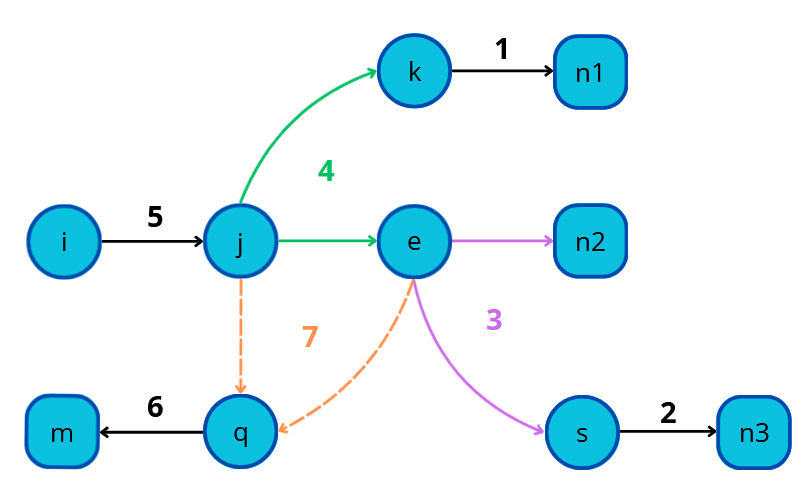
\includegraphics[width=8.4cm]{./imgs/decode_flux.PNG}
  \caption{Etapas de decodificação do fluxo na cadeia de suprimentos}
  \label{fig:decode_flux}
  \end{center}
\end{figure}

Para a decodificação de cada fluxo da cadeia de suprimentos, utilizamos a função decodingStep. Este procedimento corresponde exatamente ao Procedure 1 apresentado na Fig. 3 do artigo \cite{b12}. 
Trata-se de um algoritmo de transporte baseado em prioridades, no qual as unidades de produto são alocadas sucessivamente a partir da fonte ou destino de maior prioridade, de acordo com o vetor cromossomo. 
Em cada iteração, seleciona-se a fonte ou destino mais prioritário e realiza-se a alocação para o nó adjacente de menor custo, respeitando as restrições de capacidade e demanda. O processo se repete até que 
todas as demandas sejam atendidas. O fluxo completo de decodificação pode ser visto nos pseudocódigo dos Algoritmos \ref{algoDecode1} e \ref{algoDecode2}.

\begin{algorithm}
  \caption{Decodificação do cromossomo para a cadeia de suprimentos (Parte 1)}
  \label{algoDecode1}
  \begin{algorithmic}[1]
  \Procedure{Decode}{dados}
  \State \textbf{Entrada:} dados estruturados contendo:
  \State - Capacidades e demandas para todas as instalações
  \State - Custos unitários de transporte
  \State - Taxas de perda para cada estágio do processo
  \State - Demandas dos consumidores
  \State - Segmentos de cromossomo ($S_1, S_2, \ldots, S_8$) representando prioridades de transporte
  \State \textbf{Saída:} custototal, variáveis de decisão contínuas ($X, P, L, O, O_c, G_o, G_r, D, G_w, O_w$) e variáveis binárias de abertura ($U, W, R, V, Y$)
  
  \State \textbf{// Passo 1: Inicializar variáveis e ler dados de entrada}
  \State custototal $\leftarrow 0$

  \State \textbf{// Passo 2: Decodificar Fábricas de Pistache → Consumidores de Pistache}
  \State $a_1 \leftarrow$ capacidades das fábricas de pistache
  \State $b_1 \leftarrow$ demandas dos consumidores de pistache
  \State $c_1 \leftarrow$ custos de transporte
  \State $(custo1, P) \leftarrow \text{decodingStep}(S_1, a_1, b_1, c_1)$
  \State custototal $\leftarrow$ custototal + custo1
  
  \State \textbf{// Passo 3: Decodificar Fábricas de Cosméticos → Consumidores de Cosméticos}
  \State $a_2 \leftarrow$ capacidades das fábricas de cosméticos
  \State $b_2 \leftarrow$ demandas dos consumidores de cosméticos
  \State $c_2 \leftarrow$ custos de transporte
  \State $(custo2, L) \leftarrow \text{decodingStep}(S_2, a_2, b_2, c_2)$
  \State custototal $\leftarrow$ custototal + custo2
  
  \State \textbf{// Passo 4: Decodificar Centros de Extração de Óleo → (Consumidores de Óleo + Fábricas de Cosméticos)}
  \State $a_3 \leftarrow$ capacidades dos centros de extração de óleo
  \State $b_3 \leftarrow$ demandas dos consumidores de óleo e fábricas de cosméticos
  \State $c_3 \leftarrow$ custos de transporte
  \State $(custo3, OO_c) \leftarrow \text{decodingStep}(S_3, a_3, b_3, c_3)$
  \State Separar $OO_c$ em $O$ (consumidores de óleo) e $O_c$ (fábricas de cosméticos)
  \State custototal $\leftarrow$ custototal + custo3
  
  \State \textbf{// Passo 5: Decodificar Centro de Processamento → Fábricas de Pistache}
  \State $a_4 \leftarrow$ capacidades dos centros de processamento
  \State $b_4 \leftarrow$ demandas ajustadas das fábricas de pistache
  \State $c_4 \leftarrow$ custos de transporte
  \State $(\_\_, G_o) \leftarrow \text{decodingStep}(S_4, a_4, b_4, c_4)$
  
  \State \textbf{// Passo 6: Decodificar Centro de Processamento → Centros de Extração de Óleo}
  \State $a_5 \leftarrow$ capacidades dos centros de processamento
  \State $b_5 \leftarrow$ demandas ajustadas dos centros de extração de óleo
  \State $c_5 \leftarrow$ custos de transporte
  \State $(\_\_, G_r) \leftarrow \text{decodingStep}(S_5, a_5, b_5, c_5)$
  \EndProcedure
  \end{algorithmic}
\end{algorithm}

\begin{algorithm}
  \caption{Decodificação do cromossomo para a cadeia de suprimentos (Parte 2)}
  \label{algoDecode2}
  \begin{algorithmic}[1]
  \Procedure{Decode}{continuação}
  \State \textbf{// Passo 7: Ajustar demandas nos Centros de Processamento}
  \For{cada centro de processamento $j$}
      \State Calcular saídas necessárias com base nos fluxos de pistache e óleo
      \State Atualizar $G_o$ e $G_r$ para corresponder às capacidades efetivas
  \EndFor

  \State \textbf{// Passo 8: Decodificar Produtores de Pistache → Centros de Processamento}
  \State $a_6 \leftarrow$ capacidades dos produtores de pistache
  \State $b_6 \leftarrow$ demandas atualizadas nos centros de processamento
  \State $c_6 \leftarrow$ custos de transporte
  \State $(custo6, X) \leftarrow \text{decodingStep}(S_6, a_6, b_6, c_6)$
  \State custototal $\leftarrow$ custototal + custo6
    
  \State \textbf{// Passo 9: Decodificar Centros de Compostagem → Consumidores de Compostagem}
  \State $a_7 \leftarrow$ capacidades dos centros de compostagem
  \State $b_7 \leftarrow$ demandas dos consumidores de compostagem
  \State $c_7 \leftarrow$ custos de transporte
  \State $(custo7, D) \leftarrow \text{decodingStep}(S_7, a_7, b_7, c_7)$
  \State custototal $\leftarrow$ custototal + custo7
    
  \State \textbf{// Passo 10: Atribuir fluxos de resíduos}
  \State Calcular resíduos dos centros de processamento
  \State $a_8 \leftarrow$ capacidades disponíveis dos centros de compostagem
  \State $b_8 \leftarrow$ demandas de resíduos dos centros de processamento e extração de óleo
  \State $c_8 \leftarrow$ custos de transporte
  \State $(\_\_, O_w) \leftarrow \text{decodingStep}(S_8, a_8, b_8, c_8)$
  \State Atualizar custototal
    
  \State \textbf{// Passo 11: Definir variáveis binárias de abertura}
  \State $U \leftarrow$ centros de processamento abertos
  \State $W \leftarrow$ fábricas de pistache abertas
  \State $R \leftarrow$ centros de extração de óleo abertos
  \State $V \leftarrow$ fábricas de cosméticos abertas
  \State $Y \leftarrow$ centros de compostagem abertas
    
  \State \textbf{return} custototal, variáveis de decisão e variáveis binárias de abertura
  \EndProcedure
  \end{algorithmic}
\end{algorithm}

\subsection{Busca em Vizinhança Variável (VNS)}
O VNS explora o espaço de soluções alterando sistematicamente as estruturas de vizinhança \cite{b27}. O algoritmo alterna entre as fases de perturbação 
(\textit{shaking}) e busca local, aceitando novas soluções apenas se melhorarem a função objetivo. Essa abordagem tem se mostrado eficaz na resolução de problemas de otimização com restrições (\hspace{-0.03em}\cite{b9,b14,b15}).

A implementação do algoritmo VNS utilizado neste estudo está descrita no Algoritmo \ref{algoVNS}.

\begin{algorithm}
    \caption{Busca em Vizinhança Variável (VNS)}
    \label{algoVNS}
    \begin{algorithmic}[1]
    \Require Solução inicial $x$, tamanho máximo da vizinhança $k_{\text{max}}$, limite de tempo $t_{\text{max}}$
    \State \textbf{Saída:} Melhor solução encontrada $x^*$
    \State $x^ \Leftarrow x$
    \Repeat
    \State $k \Leftarrow 1$
    \Repeat
    \State $x' \Leftarrow \text{Shake}(x, k)$
    \State $x'' \Leftarrow \text{LocalSearch}(x')$
    \If{$f(x'') < f(x^)$}
    \State $x^ \Leftarrow x''$, $k \Leftarrow 1$
    \Else
    \State $k \Leftarrow k + 1$
    \EndIf
    \Until{$k > k_{\text{max}}$}
    \State $t \Leftarrow \text{CpuTime}()$
    \Until{$t > t_{\text{max}}$}
    \end{algorithmic}
\end{algorithm}

\subsection{Estruturas de Vizinhança}
Quatro operadores clássicos de vizinhança \cite{b7}, ilustrados na Figura \ref{fig:nbdh_op}, são utilizados para aumentar a diversidade das soluções:

\begin{itemize}
\item \textbf{Swap:} Permuta dois elementos no cromossomo.
\item \textbf{Reversion:} Inverte a sequência de elementos entre dois índices selecionados \cite{b17}.
\item \textbf{Insertion:} Move um elemento para uma nova posição, deslocando os demais conforme necessário \cite{b16}.
\item \textbf{Slide:} Remove um elemento, desloca os outros e o reinsere em uma nova posição.
\end{itemize}

Cada operação é aplicada a um vetor de prioridade selecionado aleatoriamente dentro do conjunto de soluções, garantindo a viabilidade e aumentando a eficiência da busca.

\begin{figure}[h!]
  \begin{center}
  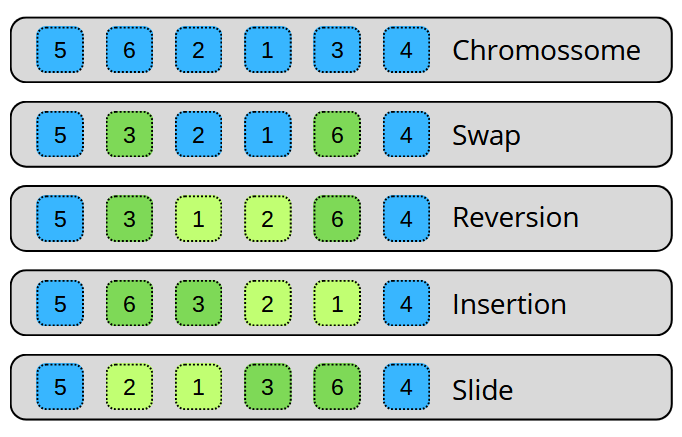
\includegraphics[width=8.4cm]{./imgs/nbhd_op.png}
  \caption{Estruturas de vizinhança utilizadas no algoritmo VNS}
  \label{fig:nbdh_op}
  \end{center}
\end{figure}

%===============================================================================
\section{Experimentos Computacionais}
\label{sec:experiments1}

O método heurístico proposto foi testado em instâncias de diferentes tamanhos, definidos pelo número de elementos em cada entidade do problema ($I$, $J$, $K$, $E$, $S$, $Q$, $N_1$, $N_2$, $N_3$ e $M$).
Os tamanhos testados foram 100, 200, 400, 800 e 1600, resultando em contagens totais de variáveis de 100.500; 401.000; 1.602.000; 6.404.000; e 25.608.000, respectivamente.
Entretanto, algoritmos que utilizam codificação baseada em prioridade possuem um número significativamente menor de variáveis, pois consideram apenas as prioridades dos pares fonte-depósito.
Nesses casos, as contagens de variáveis foram reduzidas para 1.700; 3.400; 6.800; 13.600; e 27.200.

Os parâmetros das instâncias, como capacidades e demandas, foram gerados aleatoriamente conforme a Tabela 7 de \cite{b2}. A abordagem baseada no VNS foi comparada com o GA,
que foi uma das meta-heurísticas evolucionárias utilizadas na referência considerada. O GA utilizou mutações baseadas em troca (\textit{swap-based mutations}) e cruzamentos de subsequências (\textit{subsequence-exchanging crossovers}),
com vetores selecionados aleatoriamente, uma população de 100 indivíduos e uma estratégia de seleção por Torneio Binário.

Tanto o VNS quanto o GA foram executados 30 vezes por instância. O critério de parada adotado foi um número máximo de avaliações da função objetivo, definido empiricamente de acordo 
com a complexidade de cada instância. Os valores foram escolhidos com base em testes preliminares, buscando equilibrar custo computacional e qualidade das soluções obtidas. 
Especificamente, foram utilizadas 6.250 avaliações para as instâncias de tamanho 100; 12.500 para as de tamanho 200; 25.000 para as de 400; 500.000 para as de 800; e 100.000 
para as de 1600. Adicionalmente, o VNS também pode parar a execucação quando todos os operadores de vizinhança falharem em melhorar a solução atual.

Os experimentos foram conduzidos em um sistema com Ubuntu 24.04.1 LTS, processador Intel Xeon E3-1240 V2 (8 núcleos) e 32 GB de RAM.

\subsection{Comparação entre VNS e GA}

A comparação com o GA segue a metodologia de \cite{b2}, embora uma correspondência exata não tenha sido possível devido às diferenças no processo de decodificação. 
A Tabela \ref{tab:comparison_vns_ga} apresenta o desempenho médio das 30 melhores soluções obtidas por cada algoritmo. Para instâncias pequenas (tamanho 100), o 
VNS superou o GA com uma melhoria de 4,48\%. À medida que o tamanho do problema aumentou, essa superioridade se manteve e, em alguns casos, foi ainda mais acentuada.
O VNS apresentou melhorias variando de 4,48\% a 9,87\% em relação ao GA nas instâncias maiores, com destaque para o ganho de 9,87\% na instância de 200 elementos.

\begin{table*}[!htb]
  \caption{Comparação entre o algoritmo VNS e uma meta-heurística baseada em população (GA) em termos do valor médio da função objetivo das melhores soluções e do tempo médio de execução.}
  \label{tab:comparison_vns_ga}
  \begin{tabular*}{\textwidth}{@{\extracolsep\fill}lcccccc}
  \toprule%
  & \multicolumn{3}{@{}c@{}}{Avaliação da função objetivo (média)} & \multicolumn{3}{@{}c@{}}{Tempo de Execução (média)} \\\cmidrule{2-4}\cmidrule{5-7}%
  Instância & VNS & GA & Diferença (\%) & VNS & GA & Diferença (\%) \\
  \midrule
  100  & $7.44 \times 10^7$  & $7.78 \times 10^7$  & 4.48 & 369.59s    & 60,480.38s  & 197.57 \\
  200  & $1.51 \times 10^8$  & $1.66 \times 10^8$  & 9.87 & 1,192.69s  & 23,210.39s  & 180.45 \\
  400  & $3.12 \times 10^8$  & $3.42 \times 10^8$  & 9.17 & 3,917.46s  & 27,590.31s  & 150.27 \\
  800  & $6.58 \times 10^8$  & $7.08 \times 10^8$  & 7.36 & 11,512.24s & 48,803.09s  & 123.65 \\
  1600 & $1.36 \times 10^9$  & $1.43 \times 10^9$  & 4.64 & 17,767s & 217,958s  & 1126.95 \\
  \bottomrule 
  \end{tabular*}
\end{table*}

% Os boxplots na Fig. \ref{fig:VNSxGA_boxplots} ilustram a distribuição das soluções, destacando diferenças significativas nos casos de 800 e 1600 instâncias. Os valores de p obtidos no teste t para amostras 
% independentes (teste de Welch) para essas instâncias são inferiores a 0.05, indicando que as diferenças observadas são estatisticamente significativas, considerando normalidade e variâncias desiguais. 
% Esses resultados sugerem que o VNS tem um desempenho significativamente superior ao GA em problemas de grande escala do ponto de vista estatístico. Além disso, o GA apresentou tempos de execução muito mais 
% longos, provavelmente devido ao aumento dos custos computacionais de suas operações evolutivas à medida que o tamanho do problema crescia.

% Os boxplots na Fig. \ref{fig:VNSxGA_boxplots} ilustram a distribuição das soluções, com diferenças mais significativas nas instâncias maiores.
% Esses resultados sugerem que o VNS tem um desempenho superior ao GA em problemas de grande escala. Além disso, o GA apresentou tempos de execução muito mais 
% longos, provavelmente devido ao critério de parada adicional do VNS, que leva em consideração o esgotamento dos operadores de vizinhança, enquanto o GA depende de um número fixo de avaliações da função objetivo.
% Ao mesmo tempo, isso sugere que o VNS pode estar sendo mais eficiente em encontrar soluções do ponto de vista da função objetivo com um número menor de avaliações.

Os boxplots na Fig. \ref{fig:VNSxGA_boxplots} ilustram a distribuição das soluções, com diferenças mais significativas nas instâncias maiores. Esses resultados 
sugerem que o VNS tem um desempenho superior ao GA em problemas de grande escala. Além disso, o GA apresentou tempos de execução muito mais longos, provavelmente 
devido ao critério de parada adicional do VNS, que leva em consideração o esgotamento dos operadores de vizinhança, enquanto o GA depende de um número fixo de 
avaliações da função objetivo. Ao mesmo tempo, isso sugere que o VNS pode estar sendo mais eficiente em encontrar boas soluções com um número menor de avaliações. 

Os testes estatísticos apresentados na Tabela \ref{tab:estatisticas_tests} reforçam essas observações: nas instâncias 800 e 1600, ambas as distribuições passaram no teste de normalidade de Shapiro-Wilk 
($p > 0.05$), permitindo o uso do teste t de Welch, que indicou diferenças estatisticamente significativas ($p < 0{,}05$). Já nas demais instâncias, pelo menos 
uma das distribuições não seguiu normalidade, sendo aplicado o teste de Mann-Whitney, que também revelou diferenças significativas. Assim, conclui-se que o VNS 
foi consistentemente mais eficaz estatisticamente, especialmente à medida que o tamanho do problema aumentou.

\begin{table*}[!htb]
  \caption{Resultados dos testes estatísticos para as instâncias analisadas. Inclui o p-valor do teste de normalidade (Shapiro-Wilk) para o GA e o VNS, e o teste de comparação adequado (Mann-Whitney ou t-teste), com seus respectivos p-valores.}
  \label{tab:estatisticas_tests}
  \centering
  \begin{tabular}{cccccc}
    \toprule
    Instância & Shapiro GA (p-valor) & Shapiro VNS (p-valor) & Teste Comparativo & p-valor do Teste \\
    \midrule
    100  & 0.00039   & $1.77 \times 10^{-8}$ & Mann-Whitney & $2.80 \times 10^{-7}$ \\
    200  & 0.8845    & 0.0193                & Mann-Whitney & $2.04 \times 10^{-11}$ \\
    400  & 0.0112    & 0.4451                & Mann-Whitney & $5.47 \times 10^{-11}$ \\
    800  & 0.6487    & 0.1659                & t-teste      & $4.05 \times 10^{-17}$ \\
    1600 & 0.2945    & 0.5287                & t-teste      & $1.84 \times 10^{-14}$ \\
    \bottomrule
  \end{tabular}
\end{table*}

Em resumo, embora o GA tenha um desempenho competitivo em instâncias pequenas, sua escalabilidade é limitada. Em contraste, o VNS não apenas obtém soluções superiores,
mas também demonstra maior eficiência no tratamento de problemas de grande escala, estabelecendo-se como um método de otimização mais robusto e escalável.

\begin{figure*}[h!]
  \centering
  \begin{tabular}{cc}
      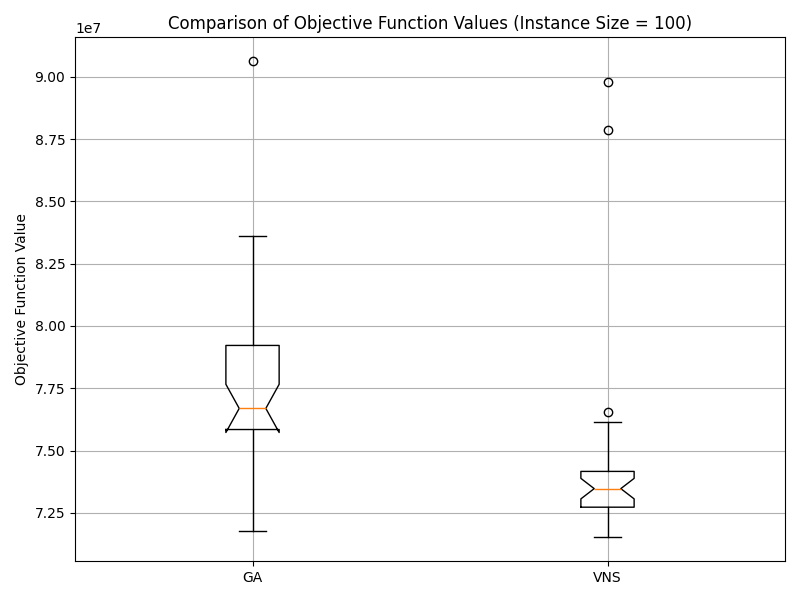
\includegraphics[width=0.45\textwidth]{./imgs/GAxVNS_100.png} & 
      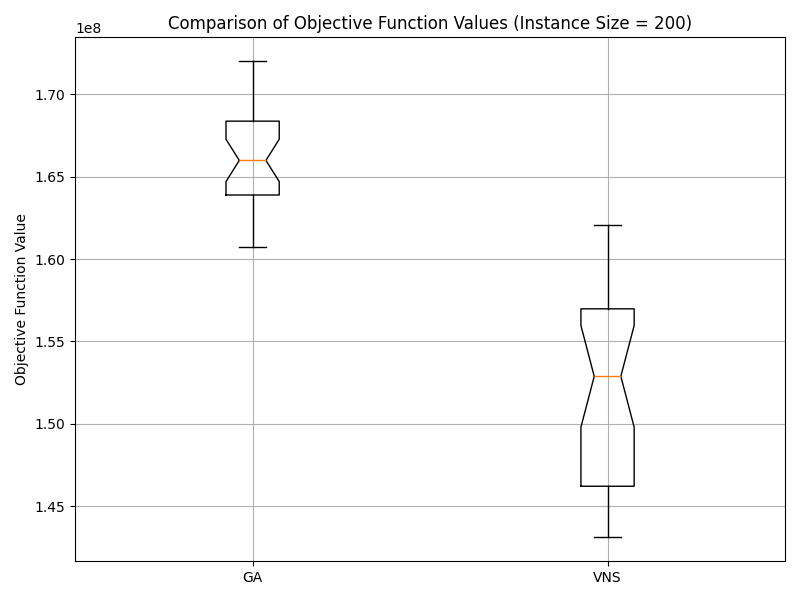
\includegraphics[width=0.46\textwidth]{./imgs/GAxVNS_200.png} \\
      (a) $I, J, K, E, S, Q, N1, N2, N3, M = 100$ & 
      (b) $I, J, K, E, S, Q, N1, N2, N3, M = 200$ \\
      \vspace{0.5cm} \\ 
      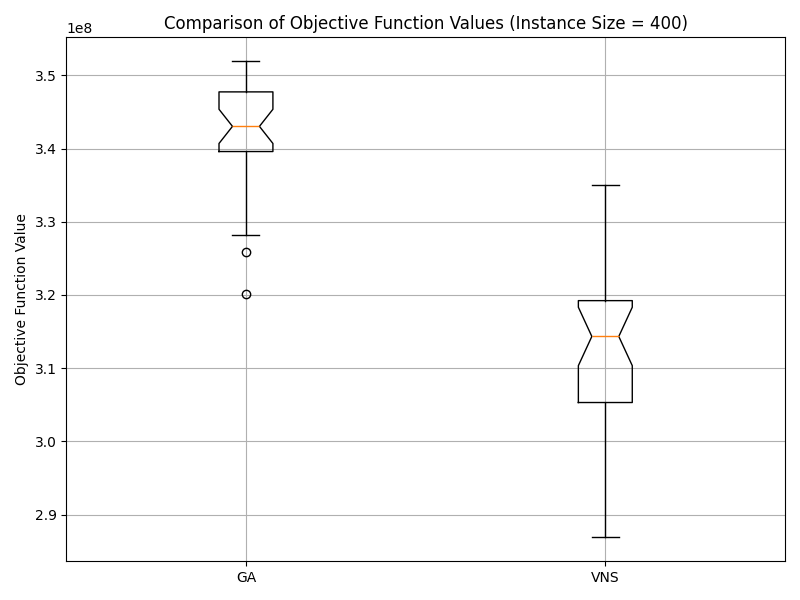
\includegraphics[width=0.47\textwidth]{./imgs/GAxVNS_400.png} & 
      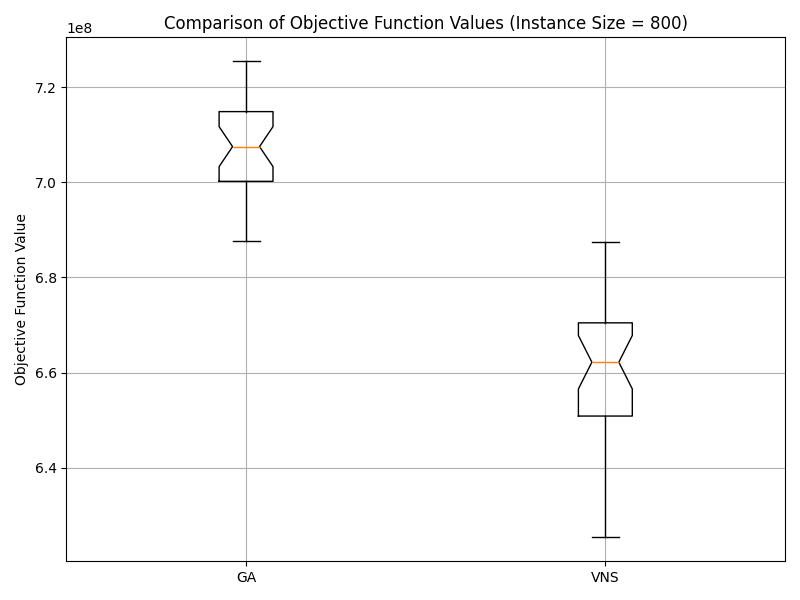
\includegraphics[width=0.45\textwidth]{./imgs/GAxVNS_800.png} \\
      (c) $I, J, K, E, S, Q, N1, N2, N3, M = 400$ & 
      (d) $I, J, K, E, S, Q, N1, N2, N3, M = 800$ \\
      \vspace{0.5cm} \\ 
      \multicolumn{2}{c}{
          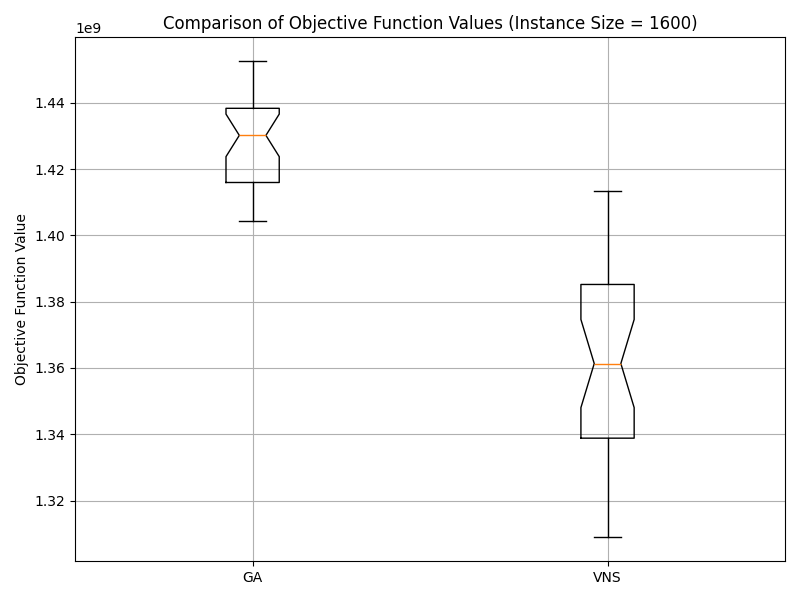
\includegraphics[width=0.45\textwidth]{./imgs/GAxVNS_1600.png} 
      } \\
      \multicolumn{2}{c}{(e) $I, J, K, E, S, Q, N1, N2, N3, M = 1600$} \\
  \end{tabular}
  \caption{Boxplots comparando o desempenho do algoritmo VNS e de uma meta-heurística baseada em população (GA) em diferentes tamanhos de problema, com base nos valores da função objetivo.}
  \label{fig:VNSxGA_boxplots}
\end{figure*}

%===============================================================================

\section{Conclusão}
\label{sec:conclusion1}

Este estudo apresenta um modelo de otimização para a cadeia de suprimentos de pistache, abordando as complexidades do gerenciamento de produtos e subprodutos ao longo de múltiplas etapas. 
Ao integrar produção, transporte e operações das instalações, o modelo garante uma alocação eficiente de recursos, respeitando as restrições de capacidade e demanda. Formulado como um problema 
de Programação Linear Inteira Mista (MILP), ele é resolvido por meio do algoritmo VNS, que explora o espaço de soluções utilizando estruturas de vizinhança como Swap, Reversion, Insertion e Slide.

A análise comparativa demonstra a superioridade do VNS em relação ao GA, tanto em qualidade das soluções quanto em eficiência computacional, especialmente para 
instâncias de grande escala, onde métodos exatos se tornam inviáveis devido a limitações de tempo e memória.

Pesquisas futuras podem explorar operadores de vizinhança específicos para o problema, aprimorando ainda mais o desempenho do VNS. Além disso, uma abordagem híbrida, combinando VNS com métodos 
exatos, pode melhorar tanto a precisão quanto a eficiência da solução, tornando a metodologia mais aplicável a diferentes setores.

O código e conjunto de dados utilizados neste estudo estão disponíveis em: \url{https://github.com/raissagd/Pistachio_CLSC}.

%===============================================================================

\begin{thebibliography}{00}
    \bibitem{b1} M. Gen, F. Altiparmak, and L. Lin, "A genetic algorithm for two-stage transportation problem using priority-based encoding," OR Spectrum, vol. 28, pp. 337--354, 2006.
    \bibitem{b2} A. Rajabi-Kafshgar, F. Gholian-Jouybari, I. Seyedi, and M. Hajiaghaei-Keshteli, "Utilizing hybrid metaheuristic approach to design an agricultural closed-loop supply chain network," Expert Syst. Appl., vol. 217, p. 119504, 2023.
    \bibitem{b3} M. K. Doula, P. Kouloumbis, and K. Elaiopoulos, "Turning wastes into valuable materials: Valorization of pistachio wastes in agricultural sector," in SYMBIOSIS Int. Conf., pp. 19--21, 2014.
    \bibitem{b4} G. Bartzas and K. Komnitsas, "Life cycle analysis of pistachio production in Greece," Sci. Total Environ., vol. 595, pp. 13--24, 2017.
    \bibitem{b5} R. Casper and E. Sundin, "Reverse logistic transportation and packaging concepts in automotive remanufacturing," Procedia Manuf., vol. 25, pp. 154--160, 2018.
    \bibitem{b6} A. Cheraghalipour and E. Roghanian, "A bi-level model for a closed-loop agricultural supply chain considering biogas and compost," Environ. Dev. Sustain., pp. 1--47, 2022.
    \bibitem{b7} K. Devika, A. Jafarian, and V. Nourbakhsh, "Designing a sustainable closed-loop supply chain network based on triple bottom line approach: A comparison of metaheuristics hybridization techniques," Eur. J. Oper. Res., vol. 235, no. 3, pp. 594--615, 2014.
    \bibitem{b8} M. Zohal and H. Soleimani, "Developing an ant colony approach for green closed-loop supply chain network design: a case study in gold industry," J. Clean. Prod., vol. 133, pp. 314--337, 2016.
    \bibitem{b9} E. K. Burke, J. Li, and R. Qu, "A hybrid model of integer programming and variable neighbourhood search for highly-constrained nurse rostering problems," Eur. J. Oper. Res., vol. 203, no. 2, pp. 484--493, 2010.
    \bibitem{b10} C. C. Ribeiro, D. Aloise, T. F. Noronha, C. Rocha, and S. Urrutia, "An efficient implementation of a VNS/ILS heuristic for a real-life car sequencing problem," Eur. J. Oper. Res., vol. 191, no. 3, pp. 596--611, 2008.
    \bibitem{b11} M. S. Pishvaee, R. Z. Farahani, and W. Dullaert, "A memetic algorithm for bi-objective integrated forward/reverse logistics network design," Comput. Oper. Res., vol. 37, no. 6, pp. 1100--1112, 2010.
    \bibitem{b12} F. Altiparmak, M. Gen, L. Lin, and T. Paksoy, "A genetic algorithm approach for multi-objective optimization of supply chain networks," Comput. Ind. Eng., vol. 51, no. 1, pp. 196--215, 2006.
    \bibitem{b13} J. Liu, B. Sun, G. Li, and Y. Chen, "An integrated scheduling approach considering dispatching strategy and conflict-free route of AMRs in flexible job shop," Int. J. Adv. Manuf. Technol., vol. 127, no. 3, pp. 1979--2002, 2023.
    \bibitem{b14} A. Imran, S. Salhi, and N. A. Wassan, "A variable neighborhood-based heuristic for the heterogeneous fleet vehicle routing problem," Eur. J. Oper. Res., vol. 197, no. 2, pp. 509--518, 2009.
    \bibitem{b15} K. Fleszar and K. S. Hindi, "An effective VNS for the capacitated p-median problem," Eur. J. Oper. Res., vol. 191, no. 3, pp. 612--622, 2008.
    \bibitem{b16} M. Rabiee, M. Zandieh, and A. Jafarian, "Scheduling of a no-wait two-machine flow shop with sequence-dependent setup times and probable rework using robust meta-heuristics," Int. J. Prod. Res., vol. 50, no. 24, pp. 7428--7446, 2012.
    \bibitem{b17} B. Vahdani and M. Zandieh, "Scheduling trucks in cross-docking systems: Robust meta-heuristics," Comput. Ind. Eng., vol. 58, no. 1, pp. 12--24, 2010.
    \bibitem{b18} M. S. Pishvaee, J. Razmi, and S. A. Torabi, "An accelerated Benders decomposition algorithm for sustainable supply chain network design under uncertainty: A case study of medical needle and syringe supply chain," Transp. Res. Part E: Logist. Transp. Rev., vol. 67, pp. 14--38, 2014.
    \bibitem{b19} S. Ahmadi and S. H. Amin, "An integrated chance-constrained stochastic model for a mobile phone closed-loop supply chain network with supplier selection," J. Clean. Prod., vol. 226, pp. 988--1003, 2019.
    \bibitem{b20} M. Banasik, A. Stanisławska-Sachadyn, and P. Sachadyn, "A simple modification of PCR thermal profile applied to evade persisting contamination," J. Appl. Genet., vol. 57, pp. 409--415, 2016.
    \bibitem{b21} F. Gholian-Jouybari, O. Hashemi-Amiri, B. Mosallanezhad, and M. Hajiaghaei-Keshteli, "Metaheuristic algorithms for a sustainable agri-food supply chain considering marketing practices under uncertainty," Expert Syst. Appl., vol. 213, p. 118880, 2023.
    \bibitem{b22} Statista, "Leading producers of pistachios worldwide in 2022 and 2023," 2023. [Online]. Available: \url{https://www.statista.com/statistics/933042/global-pistachio-production-by-country/}
    \bibitem{b23} Y. Xie, Y. Sheng, M. Qiu, and F. Gui, "An adaptive decoding biased random key genetic algorithm for cloud workflow scheduling," Eng. Appl. Artif. Intell., vol. 112, p. 104879, 2022.
    \bibitem{b24} Fathollahi-Fard, A. M., \& Hajiaghaei-Keshteli, M. (2018). A stochastic multi-objective model for a closed-loop supply chain with environmental considerations. \textit{Applied Soft Computing}, \textit{69}, 232--249.
    \bibitem{b25} Hokmabadi, H. (2018). Pistachio wastes in Iran and the potential to recapture them in value chain. \textit{Pistachio and Health Journal}, \textit{1}(4), 1--12.
    \bibitem{b26} Dronavalli, S., \& Kang, M. S. (2019). Microgametophytic selection for identifying maize with resistance to \textit{Aspergillus spp.} and aflatoxin. \textit{Journal of Crop Improvement}, \textit{33}(3), 363--371.
    \bibitem{b27} M. Gendreau and J.-Y. Potvin, Eds., Handbook of Metaheuristics, 2nd ed. Springer, 2010.    
    \bibitem{b28} P. Hansen, N. Mladenović, and J. A. Moreno Perez, "Variable neighbourhood search: methods and applications," Ann. Oper. Res., vol. 175, pp. 367--407, 2010.
    \bibitem{b29} Campelo, F., \& Aranha, C. (2023). Lessons from the Evolutionary Computation Bestiary. \textit{Artificial Life}, \textit{29}(4), 421--432. https://doi.org/10.1162/artl\_a\_00402
    \bibitem{b30} Aranha, C., Camacho Villal{'o}n, C. L., Campelo, F., Dorigo, M., Ruiz, R., Sevaux, M., S{"o}rensen, K., \& St{"u}tzle, T. (2022). Metaphor-based metaheuristics, a call for action: the elephant in the room. \textit{Swarm Intelligence}, \textit{16}(1), 1--6.
    \bibitem{b31} Gurobi Optimization, LLC, "Gurobi Optimizer Reference Manual," 2024. [Online]. Available: https://www.gurobi.com
\end{thebibliography}

\vspace{12pt}

\end{document}
